% ---
\section{\emph{Random Forest}}


\subsection{Árvores}

% ---
Árvores são modelos presentes tanto em computação como estrutura de dados e em estatística como estrutura para tomadas de decisão. No contexto de \emph{Machine Learning}, a árvore de decisão refere-se a uma estrutura de modelo preditivo, um método de aprendizagem supervisionada não parametrizada utilizada para classificação (para variáveis categóricas) e regressão (variáveis métricas). Trata-se de um modelo de conjunto de decisões ou regras na qual estabelece um fluxo dentro de sua estrutura, definindo uma classificação ou uma predição. Para \citeonline[p. 305]{HASTIE}, as árvores permitem um particionamento do espaço em um conjunto regiões. Suponha que exista \begin{math}M\end{math} partição que possa ser divida em regiões \begin{math}R_{1}, R_{2}, ..., R_{M} \end{math} e que seja possível modelar a resposta para cada região com a constante \begin{math}c_{m}\end{math}, 

\begin{equation}
f(x) = \sum_{m=1}^{M}c_{m}I( x \in R_{m} )
\end{equation}

Para a repartição dessas regiões, são definidos critérios para decidir de qual lado o dado irá ficar na árvore. São estruturas de fácil interpretação pois, uma vez criado o modelo, percorrer os nós da árvore indica as características do dado.


\tikzset{
  treenode/.style = {shape=rectangle, rounded corners,
                     draw, align=center,
                     top color=white, bottom color=blue!20},
  root/.style     = {treenode, font=\Large, bottom color=purple!30},
  env/.style      = {treenode, font=\ttfamily\normalsize},
  dummy/.style    = {circle,draw}
}

\begin{figure}[!ht]
\caption{Exemplo de árvore classificadora}
\centering
        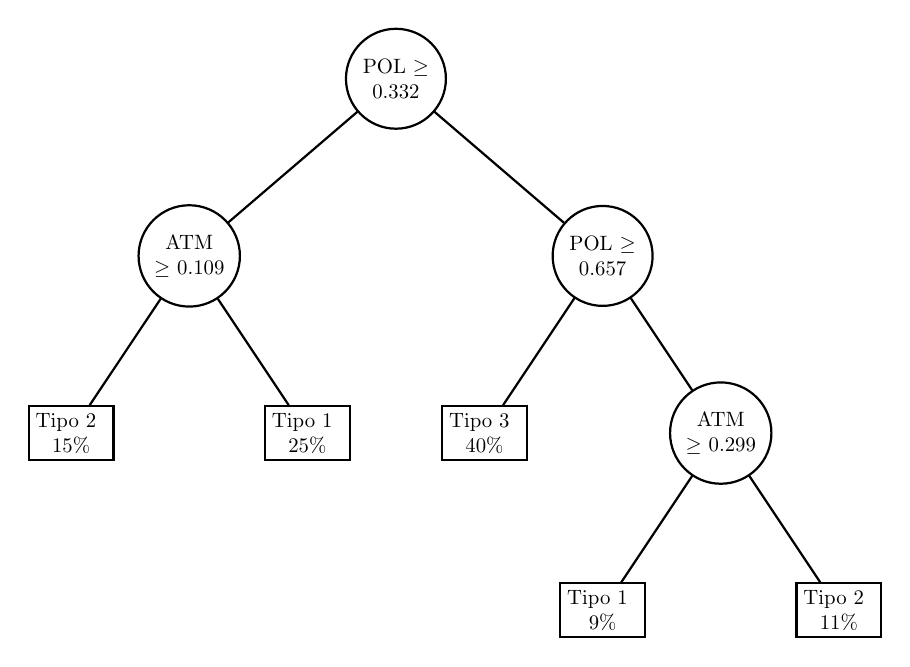
\begin{tikzpicture}[thick,scale=0.75, every node/.style={scale=0.75}]
\node [circle,draw,text width=1.2cm,align=center]{POL $\ge$ 0.332} [level distance=30mm,sibling distance=70mm]
child {node [circle,draw,text width=1.2cm,align=center] {ATM $\ge$ 0.109 } [level distance=30mm ,sibling distance=40mm]
child {node [rectangle,draw,text width=1.2cm,align=center] {Tipo 2\newline15\%}}
child {node [rectangle,draw,text width=1.2cm,align=center] {Tipo 1\newline25\%}}
}
child { node [circle,draw,text width=1.2cm,align=center]{ POL $\ge$ 0.657} [level distance=30mm ,sibling distance=40mm]
child {node [rectangle,draw,text width=1.2cm,align=center] {Tipo 3\newline40\%}}
child { node [circle,draw,text width=1.2cm,align=center]{ ATM $\ge$ 0.299 } [level distance=30mm ,sibling distance=40mm]
child {node [rectangle,draw,text width=1.2cm,align=center] {Tipo 1\newline9\%}}
child {node [rectangle,draw,text width=1.2cm,align=center] {Tipo 2\newline11\%}}
}
};
\end{tikzpicture}
\nota{Cada nó representa um atributo de um elemento da amostra. As folhas são consideradas a representação da classe a que uma observação pertence. Já o ramo é um conjunto de valores que reflete todas suas características e detalhes de um elemento}
\end{figure}

\subsubsection{Árvore de regressão}

Para \citeonline[p. 307]{HASTIE}, árvores de regressão são utilizadas em problemas de predição. Assim, a variável de saída refere-se a uma variável numérica e contínua.

Assim como foi visto anteriormente, o algoritmo deve conseseguir decidir em quais variáveis e quais pontos as decisões serão tomadas, construindo a topologia da árvore.

No caso de uma regressão, poderia utiliza-se como critério de minimização a soma do mínimos quadrados \begin{math}\sum{ (y_{i} - f(x_{i}))^{2}}\end{math}, temos que o melhor \begin{math}\hat c_{m}\end{math} é exatamente a média para \begin{math}y_{i}\end{math} na região \begin{math}R_{m}\end{math}:

\begin{equation}
\label{eq:media}
\hat c_{m} = m\acute edia(y_{i} | x_{i} \in R_{m})
\end{equation}

Para encontrar a melhor partição, é necessário recorrer a um algoritmo guloso\footnotemark \footnotetext{\emph{algoritmo guloso} é um algoritmo que  busca a resolução de um problema elegendo sempre uma solução localmente ótima. Isto significa que, dentro de um conjunto de soluções possíveis numa determinada etapa da solução do problema, escolhe-se sempre a que traz o melhor resultado naquela situação, o que muitas vezes pode não levar a uma solução ótima global.}, uma vez que calcular utilizando os mínimos quadrados é computacionalmente inviável.

Seja \begin{math}j\end{math} uma variável de reparticionamento, $s$ um ponto de divisão. É possível definir um par de semi planos 

\begin{equation}
R_{1}(j,s) = {X | X_{j}\leq s} \quad \textrm{e} \quad R_{2}(j,s) = {X | X_{j}\textgreater s})
\end{equation}

Resultando a busca pela de \begin{math}s\end{math} e \begin{math}j\end{math} que resolva

\begin{equation}
\min_{j,s} \left [ \min_{c_{1}} \sum_{x_{i} \in R_{1} (j,s)} (y_{i} - c_{1})^{2} + \min_{c_{1}} \sum_{x_{i} \in R_{2} (j,s)}(y_{i} - c_{2})^{2} \right ]
\end{equation} 


Mas como visto em \ref{eq:media}, temos que para qualquer $j$ e $s$, a minimização interna pode ser resolvida por:

\begin{equation}
\hat c_{1} = m\acute edia(y_{i} | x_{i} \in R_{1}(j,s)) \quad \textrm{e} \quad \hat c_{2} = m\acute edia(y_{i} | x_{i} \in R_{2}(j,s))
\end{equation} 

Este processo é repetido até que todas as regiões sejam descobertas.

\subsubsection{Árvore de classificação}

Para o caso de uma árvore de classificação, \citeonline[p. 308]{HASTIE} explica que o objetivo principal concentra-se em conseguir, a partir das variáveis independentes, efetuar a decisão em definir um classe para uma determinada entrada de dados. Logo, a saída é uma variável categórica.
Neste caso, utiliza-se como critério de decisão o índice de Gini\footnotemark \footnotetext{Índice de Gini mede a frequencia de que um elemento selecionado aleatoriamente de um conjunto é marcado de forma errada}
\begin{math}Gini(T) = 1 - \sum_{i=1}^{n}{ p_{i}^{2}}\end{math},
onde p é a proporção de observações de uma determinada classe para um dado nó.

\subsection{\emph{Bagging}}

As árvores vistas anteriormente são modelos interessantes de classificação mas possuem um problema: o resultado gerado por elas em geral possuem uma acurácia muito baixa quando a estrutura da árvore começa a crescer muito \cite[p. 312]{HASTIE}.
A proposta do \emph{Bagging} é criar subconjuntos dos dados, gerando diversas árvores que deverão executar a classificação. Esses modelos subconjuntos são gerados com reposição, ou seja, um mesmo dado pode estar presente em mais de um modelo no momento do treino. Cada árvore gerada fornecerá um modelo para a \emph{Random Forest} e um valor intermediário será adotado para os nós. 

\begin{figure*}[ht!]
    \centering
        \caption{Exemplo de composição da \emph{Random Forest}}
    \begin{subfigure}[t]{0.5\textwidth}
        \centering
        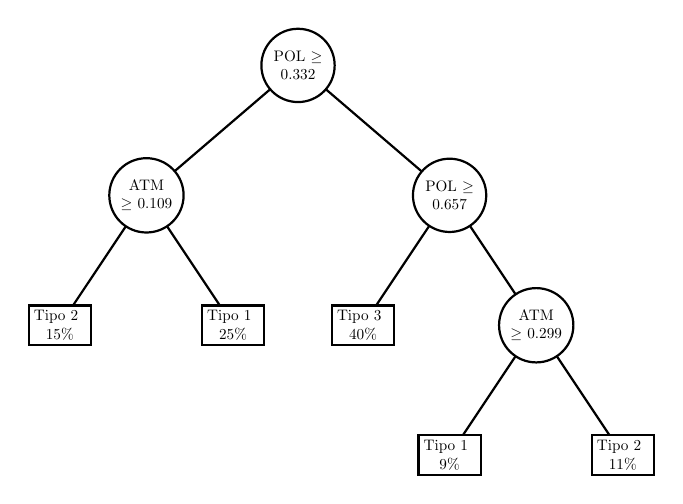
\begin{tikzpicture}[thick,scale=0.55, every node/.style={scale=0.55}]
\node [circle,draw,text width=1.2cm,align=center]{POL $\ge$ 0.332} [level distance=30mm,sibling distance=70mm]
child {node [circle,draw,text width=1.2cm,align=center] {ATM $\ge$ 0.109 } [level distance=30mm ,sibling distance=40mm]
child {node [rectangle,draw,text width=1.2cm,align=center] {Tipo 2\newline15\%}}
child {node [rectangle,draw,text width=1.2cm,align=center] {Tipo 1\newline25\%}}
}
child { node [circle,draw,text width=1.2cm,align=center]{ POL $\ge$ 0.657} [level distance=30mm ,sibling distance=40mm]
child {node [rectangle,draw,text width=1.2cm,align=center] {Tipo 3\newline40\%}}
child { node [circle,draw,text width=1.2cm,align=center]{ ATM $\ge$ 0.299 } [level distance=30mm ,sibling distance=40mm]
child {node [rectangle,draw,text width=1.2cm,align=center] {Tipo 1\newline9\%}}
child {node [rectangle,draw,text width=1.2cm,align=center] {Tipo 2\newline11\%}}
}
};
\end{tikzpicture}

        \caption{Configuração 1 da árvore de decisão}
    \end{subfigure}%
    ~ 
    \begin{subfigure}[t]{0.5\textwidth}
        \centering
        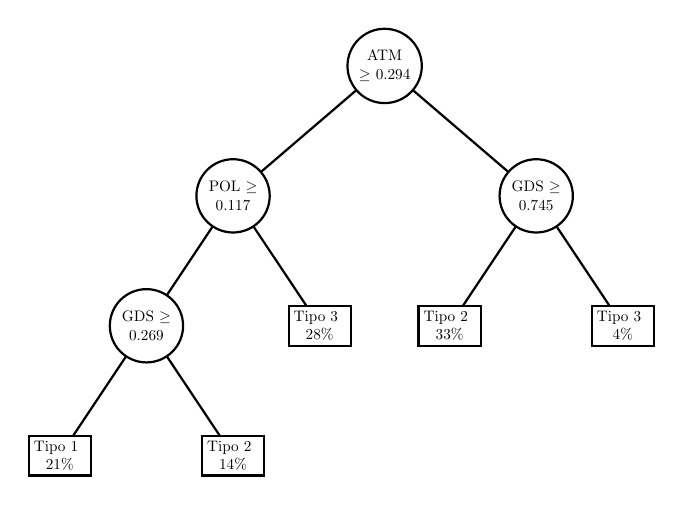
\begin{tikzpicture}[thick,scale=0.55, every node/.style={scale=0.55}]
\node [circle,draw,text width=1.2cm,align=center]{ATM $\ge$ 0.294} [level distance=30mm,sibling distance=70mm]
child { node [circle,draw,text width=1.2cm,align=center]{ POL $\ge$ 0.117 } [level distance=30mm ,sibling distance=40mm]
child { node [circle,draw,text width=1.2cm,align=center]{ GDS $\ge$ 0.269 } [level distance=30mm ,sibling distance=40mm]
child {node [rectangle,draw,text width=1.2cm,align=center] {Tipo 1\newline21\%}}
child {node [rectangle,draw,text width=1.2cm,align=center] {Tipo 2\newline14\%}}}
child {node [rectangle,draw,text width=1.2cm,align=center] {Tipo 3\newline28\%}}
}
child {node [circle,draw,text width=1.2cm,align=center] { GDS $\ge$ 0.745 } [level distance=30mm ,sibling distance=40mm]
child {node [rectangle,draw,text width=1.2cm,align=center] {Tipo 2\newline33\%}}
child {node [rectangle,draw,text width=1.2cm,align=center] {Tipo 3\newline4\%}}
};
\end{tikzpicture}
        \caption{Configuração 2 da árvore de decisão}
    \end{subfigure}

\end{figure*}



% \begin{figure*}[t!]
%     \centering
%     \begin{subfigure}[t]{0.5\textwidth}
%         \centering
%         \begin{tikzpicture}[thick,scale=0.55, every node/.style={scale=0.55}]
% \node [circle,draw,text width=1.2cm,align=center]{POL $\ge$ 0.332} [level distance=30mm,sibling distance=70mm]
% child {node [circle,draw,text width=1.2cm,align=center] {ATM $\ge$ 0.109 } [level distance=30mm ,sibling distance=40mm]
% child {node [rectangle,draw,text width=1.2cm,align=center] {Tipo 2\newline15\%}}
% child {node [rectangle,draw,text width=1.2cm,align=center] {Tipo 1\newline25\%}}
% }
% child { node [circle,draw,text width=1.2cm,align=center]{ POL $\ge$ 0.657} [level distance=30mm ,sibling distance=40mm]
% child {node [rectangle,draw,text width=1.2cm,align=center] {Tipo 3\newline40\%}}
% child { node [circle,draw,text width=1.2cm,align=center]{ ATM $\ge$ 0.299 } [level distance=30mm ,sibling distance=40mm]
% child {node [rectangle,draw,text width=1.2cm,align=center] {Tipo 1\newline9\%}}
% child {node [rectangle,draw,text width=1.2cm,align=center] {Tipo 2\newline11\%}}
% }
% };
% \end{tikzpicture}

%         \caption{Configuração 1 da árvore de decisão}
%     \end{subfigure}%
%     ~ 
%     \begin{subfigure}[t]{0.5\textwidth}
%         \centering
%         \begin{tikzpicture}[thick,scale=0.55, every node/.style={scale=0.55}]
% \node [circle,draw,text width=1.2cm,align=center]{ATM $\ge$ 0.294} [level distance=30mm,sibling distance=70mm]
% child { node [circle,draw,text width=1.2cm,align=center]{ POL $\ge$ 0.117 } [level distance=30mm ,sibling distance=40mm]
% child { node [circle,draw,text width=1.2cm,align=center]{ GDS $\ge$ 0.269 } [level distance=30mm ,sibling distance=40mm]
% child {node [rectangle,draw,text width=1.2cm,align=center] {Tipo 1\newline21\%}}
% child {node [rectangle,draw,text width=1.2cm,align=center] {Tipo 2\newline14\%}}}
% child {node [rectangle,draw,text width=1.2cm,align=center] {Tipo 3\newline28\%}}
% }
% child {node [circle,draw,text width=1.2cm,align=center] { GDS $\ge$ 0.745 } [level distance=30mm ,sibling distance=40mm]
% child {node [rectangle,draw,text width=1.2cm,align=center] {Tipo 2\newline33\%}}
% child {node [rectangle,draw,text width=1.2cm,align=center] {Tipo 3\newline4\%}}
% };
% \end{tikzpicture}
%         \caption{Configuração 2 da árvore de decisão}
%     \end{subfigure}
%     \\
%     \centering
%     \begin{subfigure}[t]{0.5\textwidth}
%         \centering
%         \begin{tikzpicture}[thick,scale=0.55, every node/.style={scale=0.55}]
% \node [circle,draw,text width=1.2cm,align=center]{POL $\ge$ 0.332} [level distance=30mm,sibling distance=70mm]
% child {node [circle,draw,text width=1.2cm,align=center] {ATM $\ge$ 0.109 } [level distance=30mm ,sibling distance=40mm]
% child {node [rectangle,draw,text width=1.2cm,align=center] {Tipo 2\newline15\%}}
% child {node [rectangle,draw,text width=1.2cm,align=center] {Tipo 1\newline25\%}}
% }
% child { node [circle,draw,text width=1.2cm,align=center]{ POL $\ge$ 0.657} [level distance=30mm ,sibling distance=40mm]
% child {node [rectangle,draw,text width=1.2cm,align=center] {Tipo 3\newline40\%}}
% child { node [circle,draw,text width=1.2cm,align=center]{ ATM $\ge$ 0.299 } [level distance=30mm ,sibling distance=40mm]
% child {node [rectangle,draw,text width=1.2cm,align=center] {Tipo 1\newline9\%}}
% child {node [rectangle,draw,text width=1.2cm,align=center] {Tipo 2\newline11\%}}
% }
% };
% \end{tikzpicture}

%         \caption{Configuração 1 da árvore de decisão}
%     \end{subfigure}%
%     ~ 
%     \begin{subfigure}[t]{0.5\textwidth}
%         \centering
%         \begin{tikzpicture}[thick,scale=0.55, every node/.style={scale=0.55}]
% \node [circle,draw,text width=1.2cm,align=center]{ATM $\ge$ 0.294} [level distance=30mm,sibling distance=70mm]
% child { node [circle,draw,text width=1.2cm,align=center]{ POL $\ge$ 0.117 } [level distance=30mm ,sibling distance=40mm]
% child { node [circle,draw,text width=1.2cm,align=center]{ GDS $\ge$ 0.269 } [level distance=30mm ,sibling distance=40mm]
% child {node [rectangle,draw,text width=1.2cm,align=center] {Tipo 1\newline21\%}}
% child {node [rectangle,draw,text width=1.2cm,align=center] {Tipo 2\newline14\%}}}
% child {node [rectangle,draw,text width=1.2cm,align=center] {Tipo 3\newline28\%}}
% }
% child {node [circle,draw,text width=1.2cm,align=center] { GDS $\ge$ 0.745 } [level distance=30mm ,sibling distance=40mm]
% child {node [rectangle,draw,text width=1.2cm,align=center] {Tipo 2\newline33\%}}
% child {node [rectangle,draw,text width=1.2cm,align=center] {Tipo 3\newline4\%}}
% };
% \end{tikzpicture}
%         \caption{Configuração 2 da árvore de decisão}
%     \end{subfigure}
%     \caption{Configurações da árvore de decisão sobre subconjuntos distintos}
% \end{figure*}

Dessa forma, a solução para contornar esse problema foi a utilização dessa técnica nas árvores de decisões. Na \emph{Random Forest}, constrói-se uma árvore de classificação repetidamente usando amostras aleatórias do conjunto de dados. Por fim, o modelo final é recalculado.
